\section{Architektur}\label{kapitel2}
\subsection{Überblick}
\begin {figure}[htb]
\centering
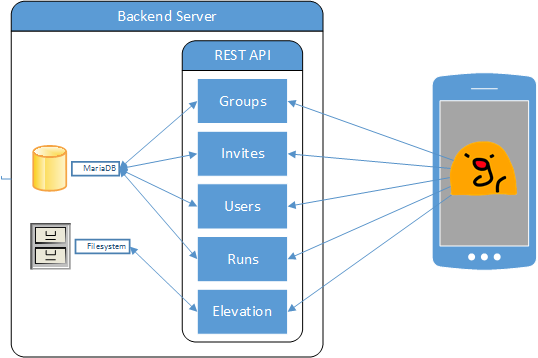
\includegraphics{abb/network_diagram_visio}
\caption{Kommunikation zwischen App und Backend-Server}
\end{figure}
Im folgenden erkläre ich die auf der Abbildung dargestellten Komponenten und warum diese für das Projekt gewählt wurden.
\subsection{Backend Server}
\subsubsection{Betriebssystem}
Bei dem Betriebssystem auf dem Backendserver handelt es sich um die Linux-Distribution Ubuntu der Version 14.04.2. Diese eignet sich besonders gut für den Einsatz auf einem möglichst dauerhaft erreichbaren Server da es sich um ein Long-Term-Support-Version handelt. Diese garantiert die Versorgung mit Sicherheits- und Wartungs-Updates für fünf Jahre ab Veröffentlichung.
\subsubsection{Datenbank}
Als Datenbankverwaltungssystem  haben wir uns entschieden ``MariaDB'' zu nutzen. MariaDB ist das Pendant zu ``MySQL'', jedoch ist es schneller, sicherer und hat eine aktivere Community.
Beide Teammitglieder könne bereits auf längere Erfahrung in MySQL zurückgreifen. Die Arbeit mit MariaDB war aufgrund des weitgehend identischen Befehlssatzes sehr unkompliziert. %HIBERNATE!
\subsubsection{REST API}
Um der App eine geeignete Schnittstelle zu Daten über das Internet bereitzustellen haben wir uns für eine REST API entschieden.
REST steht für ``Representational State Transfer'', einem stetig wachsenden Architekturmodell für Client-Server-Kommunikation bei Web Services.
\paragraph{REST Allgemein}
REST ist zustandslos, d.h. jede Nachricht enthält genügend Informationen um den Inhalt zu verstehen. Das ist besonders wichtig mit Augenmerk auf Skalierbarkeit. So ist die Lastenverteilung der REST-Anfragen auf mehrere Systeme sehr einfach, da keine sitzungspezifischen Daten o.Ä. zwischen den Servern synchronisiert werden müssen. Das gleiche gilt natürlich auch für High-Availability-Systeme.

REST schöpft den HTTP Funktionsumfang weitgehend aus, um u.A. erweitertes Caching und eine hohe Selbsterklärungsfähigkeit zu garantieren.

So erlaubt die Operation ``POST'' es, neue Ressourcen zu erstellen.

``GET'' ermöglicht es, Resourcen anzufragen. ``GET'' ist nullipotent, d.h. es werden unter Garantie keine Änderungen an der Ressource stattfinden.

Mit ``PUT'' kann man eine Ressource ersetzen, mit ``DELETE'' löschen. Diese beiden Operationen bezeichnet man als ``idempotent''. Das bedeutet dass die Anfrage das gleiche Ergebnis produzieren wird, egal wie häufig diese wiederholt wird.

Jeder Ressource ist genau eine URL zugeordnet. Beispielsweise bekommt so der Client mit einer Anfrage mit der Operation ``GET'' auf ``myserver.com/run'' die Liste aller Läufe zurück, während die gleiche Anfrage auf ``myserver.com/run/15'' nur den Lauf mit der ID 15 zurückgibt. 

Ein weitere Eigenschaft von REST ist es, dass die Kommunikationsform nicht standardisiert ist. So ist es möglich, anhand von Daten verpackt in JSON, HTML, XML oder auch in einem komplett eigenen Format zu kommunizieren.
\paragraph{Spring Framework und Tomcat}
Für die Realisierung der Webservices haben wir uns entschieden das Spring Framework zu nutzen.
Ersteres wurde gewählt da es bei einem Teammitglied relevant für die Bachelorarbeit wird und sich so in das Framework eingearbeitet werden konnte. 

Das quelloffene Framework erlaubt es u.A. skalierbare, performante, reichhaltige Web-Services aufzusetzen. Es ist möglich spezifische Sicherheitsmaßnahmen umzusetzen, JSON, XML o.Ä. automatisch zu serialisieren und deserialisieren, Anfragen zu validieren usw., d.h. es ist mehr als ausreichend für den Rahmen dieser Studienarbeit.

Die Programmierung im Spring-Framework erfolgt mit Java (mit zusätzlichen Annotationen) und XML. Es vereinfacht das Programmierprinzip Dependency Injection durch wahlweise das automatische Einlesen von hinterlegten XML-Dateien oder Annotationen im Java-Code. Auch das Programmierparadigma ``Aspektorientierte Programmierung'' wird dem Programmierer nahegelegt.
Spring besteht aus vielen kleineren Frameworks, von denen einige Verwendung im Projekt gefunden haben:
\begin{itemize}
\item Sping Core - Das ``Kern''-Framework.
\item Spring Web - Um Web-Applikationen zu erstellen.
\item Spring Web MVC - Fügt ein DispatcherServlet hinzu dass Anfragen an Handler/Controller weiterleitet und damit das MVC-Programmiermuster stark vereinfacht.\footnote{Introduction to Spring Web MVC framework, vgl.~\cite{webmvc}~[S.437]}. 
\item Spring Security - Die Sicherheitskomponente für das Spring Framework.
\end{itemize}

Als Application Server wurde Tomcat gewählt, da beide Teammitglieder diesen vorher bereits mehrfach aufsetzen durften und eventuell spätere Sicherheitsmaßnahmen wie das Einbinden eines Zertifikats um den HTTP-Verkehr über SSL zu verschlüsseln in wenigen Minuten möglich ist.
\paragraph{JSON}
Als Format für den Austausch von Daten zwischen Server und Client haben wir uns für JSON entschieden.

JSON weist im Vergleich zum stärksten Konkurrenten XML eine hohe Lesbarkeit auf und lässt sich sowohl auf dem Server als auch auf der App sehr einfach von und zu Java-Objekten serialisieren und deserialisieren.

Auf dem Server übernimmt diese Aufgabe Jackson, auf der App Gson.
\paragraph{Maven}
Das manuelle Einbinden von JARs in Java-Projekte stellt eine Herausforderung da. Hierbei müssen diese von vertrauenswürdigen Quellen manuell heruntergeladen werden, in den richtigen Ordner verschoben und importiert werden.

Um den Aufwand zu minimieren nutzen wir Maven, welche sich selbst um das Herunterladen und Einbinden der Java-Archive kümmert. Dabei ist auch das Aktualisieren der Pakete durch das Ändern einer einzigen Zeile in der Maven-Konfigurationsdatei möglich.
\subsection{App}
Die App ist für Android 5.0 ab API 21 geschrieben. 

Für das Betriebssystem Android haben wir uns entschieden da beide Teammitglieder ein Android-Smartphone besitzen. Da es sich bei dieser Studienarbeit um kein Projekt mit wirtschaftlicher Motivation handelt und die API einige Verbesserungen gegenüber älteren Versionen mitbringt hielt uns von der Entscheidung auch nicht die relativ geringe Verbreitung von 12,4\% der APIs 21 und 22 ab\footnote{Dashboards, vgl.~\cite{verbreitung}} (Stand 1. Juni 2015).